% !TEX root = ../../main.tex

\section{Context and scientific approach}



\begin{figure}[htb]
    \centering

    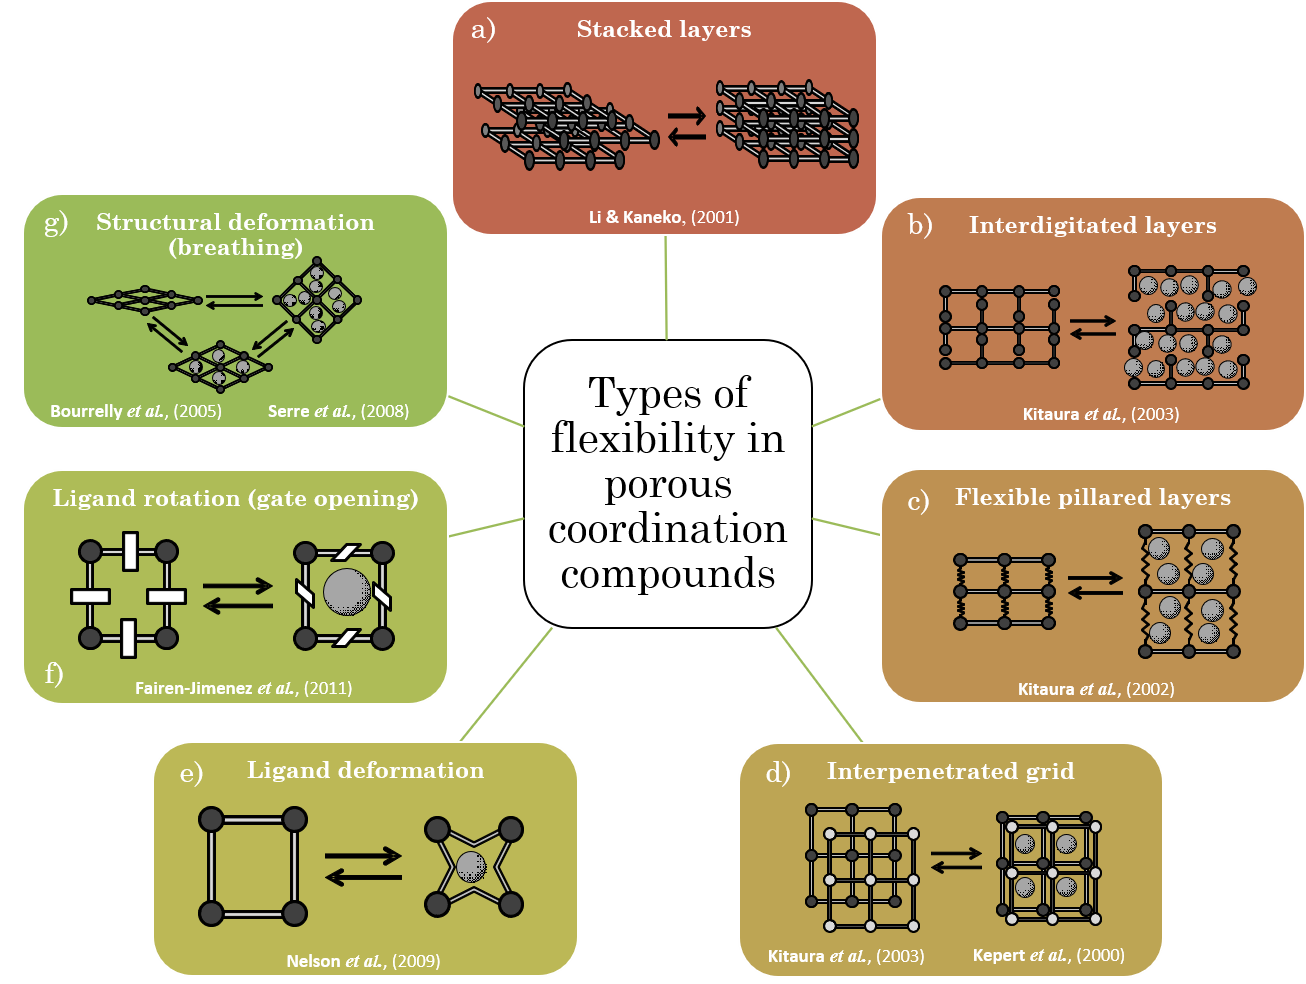
\includegraphics[width=\textwidth]{flexibility-types}%
    \caption{A visual summary of the types of flexibility
    which are documented in MOFs, as detailed in 
    (a)~\citet{liHydrogenBondregulatedMicroporous2001}
    (b)~\citet{kitauraPorousCoordinationPolymerCrystals2003}
    (c)~\citet{kitauraPillaredLayerCoordinationPolymer2002}
    (d)~\citet{kepertVersatileFamilyInterconvertible2000,%
    kitauraPorousCoordinationPolymerCrystals2003}
    (e)~\citet{nelsonSupercriticalProcessingRoute2009}
    (f)~\citet{fairen-jimenezOpeningGateFramework2011}
    (g)~\citet{bourrellyDifferentAdsorptionBehaviors2005, %
    serreExplanationVeryLarge2007}}
    
\end{figure}
